\chapter{Attacchi su blockchain}

\section{Contesto}
L'effettiva sicurezza del protocollo Bitcoin non è sempre verificabile nella pratica. Una simulazione o un effettivo attacco sulla blockchain è molto dispendioso in termini di investimenti, risorse e tempi. Nonostante le tecnologie utilizzate nella blockchain siano già conosciute, studiate e con personale esperto, non esistono molte figure professionali totalmente preparate ad affrontare queste tipologie di scenari. Le conoscenze necessarie per questo tipo di attività sono specialistiche e necessitano di esperienza, capacità e un nuovo modo di pensare. A causa di questo divario molti degli eventi di sicurezza relativi a Bitcoin o altre criptomonete non riguardano strettamente il protocollo ma i software o i servizi utilizzati. Uno dei più famosi è quello riguardante \textit{Mt. Gox} (\textit{Magic the Gathering Online Exchange}) che ha portato alla chiusura per bancarotta del servizio, la perdita di $740000$ Bitcoin\footnote{In valore in Euro è di 460 milioni.} e l'arresto del fondatore di due altri exchange\footnote{Un exchange è una piattaforma, presentata come sito web, in cui è possibile acquistare e vendere delle criptomonete o scambiare valuta corrente con criptomonete in base al rapporto domanda e offerta.} per riciclaggio di denaro.\newline
\begin{figure}
    \centering
    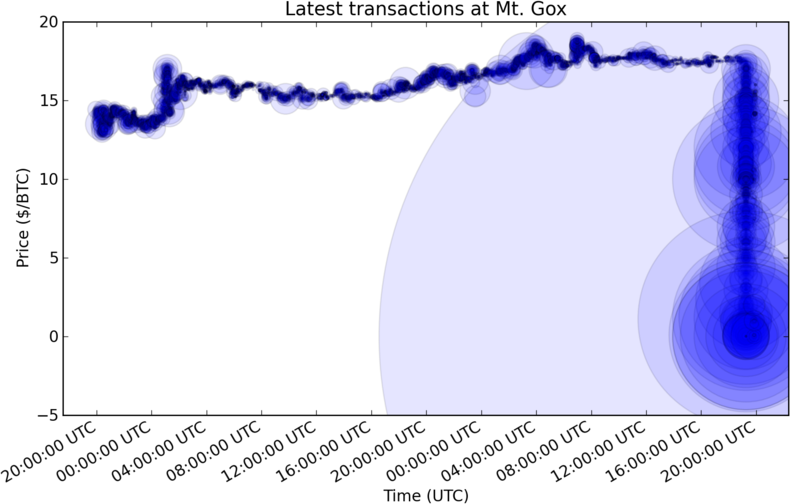
\includegraphics[width=\textwidth]{images/mtgox_cent.png}
    \caption{Crollo del prezzo dei Bitcoin durante l'hack del 2011}
    \source{Wikipedia}
\end{figure}
Nel 2014, \textit{Mt. Gox}, un \textit{exchange} con base in Giappone, gestiva complessivamente circa il $70\%$ delle transazioni mondiali su Bitcoin. \textit{Mt. Gox} fu fondato nel 2010 da \textit{Jed McCaleb} (creatore anche della più recente criptomoneta \textit{Ripple}) ma già nel 2011 un computer di una collaborazione dell'azienda fu compromesso. Gli attaccanti sfruttarono l'accesso del computer compromesso per cambiare i valori di cambio nel servizio di exchange; in questo modo gli attaccanti acquistarono $650$ Bitcoin a $0.0.1$ Euro ciascuno e vendettero circa $2000$ BTC appartenenti ad altri clienti alla stessa riadattata cifra.\newline
Successivamente a questa compromissione \textit{Mt. Gox} ha implementato diverse misure di sicurezza e fino al 2014 registrò una crescita esponenziale sfruttando anche la crescita di interesse generata dai Bitcoin. Nonostante questa prima compromissione, le misure di sicurezza applicate e l'aumento di prestigio ed utilizzo, molti furono i problemi dovuti alla gestione del servizio e delle licenze (\textit{US Department of Homeland Security} confiscò $5$ milioni di dollari come multa per trasferimento non autorizzato di moneta). In aggiunta ai problemi legali e di gestione, nel 2014 un documento dichiarò la perdita di $744408$ Bitcoin appartenenti ai clienti e $100000$ appartenuti a \textit{Mt. Gox}; una approfondita indagine scoprì che dal settembre 2011 (poco dopo la prima compromissione) ne subì un'altra, più grave, e che il servizio era insolvente già da allora. Dopo il crollo del servizio \textit{Mark Karpelés}, che comprò \textit{Mt. Gox} nel marzo 2011, fu arrestato nel 2015 e poi rilasciato per frode ed appropriazione indebita. Nel 2017 \textit{Alexander Vinnik} fu arrestato dalle autorità statunitensi in Grecia per riciclaggio di denaro derivato dal furto di Bitcoin da \textit{Mt. Gox}; l'investigazione dimostrò che i wallet utilizzati per derubare \textit{Mt. Gox} sono stati trasferiti o venduti presso l'exchange \textit{BTC-e} di proprietà di \textit{Vinnik}.\newline
Negli ultimi anni sono stati rilevati molti software per wallet creati appositamente per rubare le chiavi private degli utilizzatori; anche software creati senza scopi malevoli però possono essere soggetti ad attacchi o furti se gli algoritmi di crittografia non sono implementati correttamente; per esempio \texttt{Bitcoin Core} fu affetto dalla vulnerabilità chiamata \texttt{Heartbleed}\footnote{\url{https://bitcoin.org/en/alert/2014-04-11-heartbleed}}.\newline\newline
Gli esempi riportati e tutti gli altri maggiori problemi di sicurezza resi pubblici in questi anni non sono dovuti a falle o exploit delle blockchain o del protocollo ma a software o servizi male implementati o gestiti. Attualmente non sono noti attacchi di successo portati alla blockchain Bitcoin.\newline
Gli attacchi più distruttivi per la blockchain sono quelli riguardanti falle negli algoritmi di crittografia: una falla in \textit{SHA256} o \textit{ECDSA} sarebbe disastrosa per l'intera rete. Nonostante ciò, la possibilità che esso si verifichi è quasi nulla in quanto gli algoritmi crittografici utilizzati sono stati analizzati e testati a fondo e non hanno fatto emergere vulnerabilità critiche.

\section{Double Spending Attack e $51\%$}
Il \textit{double spending} è uno dei possibili attacchi più famosi alla rete Bitcoin e quello che fu previsto anche dallo stesso Satoshi Nakamoto. Nel paper infatti Satoshi dichiara espressamente che Bitcoin è stato creato per prevenire il \textit{double spending} in assenza di terze parti per il controllo delle transazioni.\newline
Questo tipo di attacco è esclusivo per le criptomonete e pagamenti online in quanto nel mondo fisico non sarebbe possibile replicarlo.
\begin{figure}
    \centering
    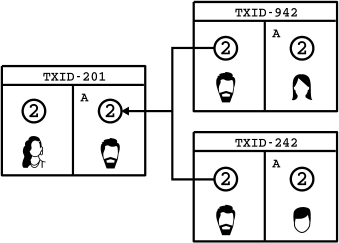
\includegraphics[width=0.5\textwidth]{images/double_spending.png}
    \caption{La transazione numero $942$ cede dei Bitcoin da Bob ad Alice tramite la \textit{UTXO} $201$ ma al tempo stesso Bob utilizza lo stesso output per una transazione verso Carol ($242$) \cite{owning}}
\end{figure}
Un \textit{double spending} avviene quando vengono create due o più transazioni diverse utilizzando la stessa \textit{UTXO} come input; questo si concretizza con la ricezione di moneta che risulta però essere già spesa. Bitcoin non implementa un modo per prevenire questo tipo di attacco a priori ma adotta un meccanismo di detection e risoluzione: solo una delle due transazioni verrà inserita, prima o poi, nella blockchain definitiva e non in alcune branch (o \textit{fork}) temporanee.\newline
L'attacco non è evitabile semplicemente avendo fiducia degli utenti e nella loro correttezza in quanto questi stessi utenti potrebbero essere stati vittima di un \textit{double spending}.\newline
Il più semplice scenario di un attacco \textit{double spending} prevede due attori, un commerciante ed un utente, che si scambiano dei Bitcoin. Bob invia dei token al commerciante in cambio di un bene o servizio. Non appena il commerciante verifica che Bob ha pubblicato la transazione nella rete e conferma l'acquisto senza aspettare che la transazione venga inserita nella blockchain o che siano stati validati almeno sei blocchi. Appena Bob riceve la conferma dell'acquisto propaga nella rete una transazione dello stesso valore verso se stesso utilizzando la stessa \textit{UTXO} utilizzata per pagare il commerciante.\newline
Una volta che entrambe le transazioni sono nella rete si crea un condizione di \textit{race condition}: se la seconda transazione di propaga più rapidamente della prima è possibile che l'attacco abbia successo in quanto i nodi implementano la policy del \textit{first seen}. I nodi che però implementano dei meccanismi di detection possono rilevare entrambe le transazioni e inviare dei messaggi di avvertimento agli altri peer.\newline
Un altro tipo di soluzione vincente per l'attaccante è quella di aver abbastanza potenza di calcolo da creare una catena di blocchi più lunga e quindi una riorganizzazione nei peer e la catena principale. Se l'attaccante ha una potenza di calcolo sufficiente da sovrastare la lunghezza della catena principale, utilizzata dalla maggior parte dei miner e dei \textit{full-node}, può inserire la seconda transazione creata nella chain creando un \textit{double spending}.\newline
Satoshi ha calcolato che la possibilità che un attaccante possa sovrastare la catena è riconducibile al problema della \textit{rovina dello scommettitore}. Uno scommettitore, con infinito budget e un deficit in partenza, gioca un numero infinito di round, la probabilità per raggiungere un pareggio nel bilancio personale è data da:
\begin{equation}
    q_{z}= \begin{cases}1, & \mbox{if }p\le q \\ (q/p)^{z}, & \mbox{if } p>q\end{cases}
\end{equation}
con $p$ la probabilità che un nodo onesto trovi il blocco successivo, $q$ la probabilità che l'attaccante trovi il blocco successivo e $q_{z}$ la probabilità che l'attaccante recuperi $z$ di svantaggio rispetto alla chain primaria. Date queste premesse se $p>q$ la probabilità decresce esponenzialmente con il divario di blocchi. Al fine di specificare la potenza di calcolo, ovvero l'hashrate, di un nodo è possibile utilizzare la distribuzione di \textit{Poisson} la probabilità di successo di un attaccante con una frazione $f$ dell'hashrate globale.
\begin{equation}\label{eq:confirmation}
    p=\sum_{k=0}^{z} \frac{\lambda^{k}*e^{-\lambda}}{k!}(1-f^{z-k})
\end{equation}
con $\lambda$ la media del numero di blocchi generati in un intervallo di tempo. La ``regola'' secondo cui una transazione è considerata confermata solo dopo sei transazioni deriva dalla formula \ref{eq:confirmation}: uno nodo con una potenza di calcolo pari al $25\%$ di quella globale ha il $5\%$ di probabilità di causare una riorganizzazione della blockchain.
\begin{figure}[H]
    \centering
    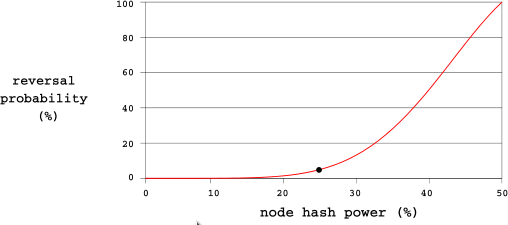
\includegraphics[width=0.9\textwidth]{images/hashrate_curve.png}
    \caption{Visualizzazione della distribuzione delle probabilità per un attaccante con $z=6$.}
\end{figure}
Dalla stessa formula è anche possibile osservare il motivo per cui il \textit{double spending} è strettamente collegato all'attacco chiamato \textit{del 51\%}. La soglia del $50\%$ è un riferimento secondo il quale un attaccante con la maggioranza del'hashrate totale possa generare blocchi più velocemente del resto dei peer. In aggiunta il nodo può anche applicare delle regole di censura e filtraggio sulle transazioni inserite nei blocchi.\newline
Nella storia dei Bitcoin non si è mai verificato un \textit{double spending} in quanto nessun nodo ha mai raggiunto una soglia tale da avere la maggioranza della computazione. Nel marzo del 2013 però, tramite un post nel forum \href{https://bitcointalk.org/index.php?topic=152348.0}{\textit{bitcointalk}}, un utente dichiara di aver, involontariamente, effettuato un \textit{double spending}.
\begin{figure}[H]
    \centering
    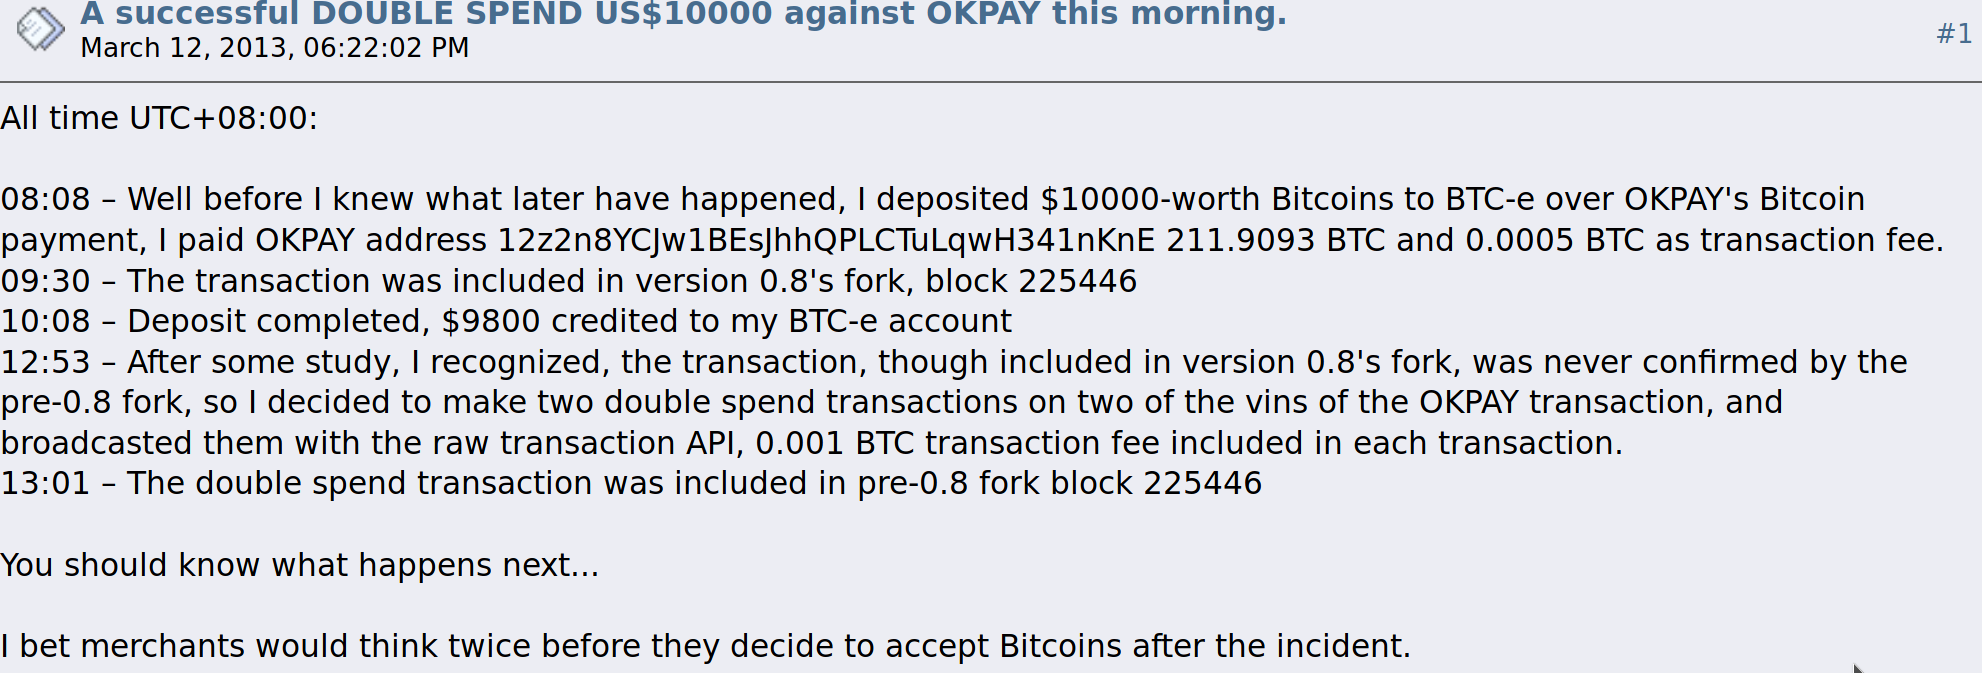
\includegraphics[width=\textwidth]{images/double_spending_post.png}
    \caption{Post pubblicato da un utente che dichiara di aver eseguito un \textit{double spending}}
    \source{\url{bitcointalk.org}}
\end{figure}
Le due transazioni effettuate dall'utente però sono state inserite a in due catene diverse a causa di una differenza di versione tra i peer della rete. Il blocco contenente la seconda transazione è stato generato e inserito nella blockchain dai nodi con la versione $0.8$ di \texttt{bitcoind} ma i nodi con una versione precedente lo hanno rifiutato. Nella rete, quindi, si sono create due \textit{fork}: una prodotta dai nodi con versione $0.8$ e una prodotta dai nodi pre-$0.8$. In quanto però i nodi con la nuova versione complessivamente avevano il $60\%$ dell'hashrate totale le due \textit{branch} non si sarebbero più riunite o aggiornate con il passare del tempo. Una soluzione a questo problema è stata quella di fare il downgrade del software dei maggiori \textit{mining pool} (\textit{BTCGuild} e \textit{Slush}); una volta che la maggioranza della potenza di calcolo è tornata alla \textit{branch} pre-$0.8$ la transazione con il \textit{double spending} è stata rifiutata (non è mai entrata nella blockchain).

\section{Forking Attack}
Il \textit{forking attack} è un attacco che ha come obiettivo effettuare un \textit{double spending} ed è strettamente collegato con la regola del $51\%$.
\begin{figure}[H]
    \centering
    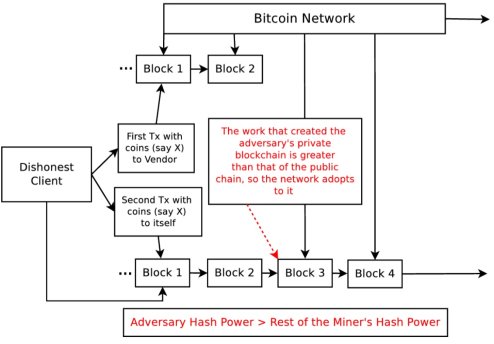
\includegraphics[width=0.75\textwidth]{images/forkingattack.png}
    \caption{Schematizzazione di un \textit{forking attack}.}
    \source{acolyer.org}
\end{figure}
L'obiettivo dell'attaccante è sviluppare la branch con la seconda transazione del \textit{double spending} in modo tale che diventi la più lunga e prevalga sull'altra. Una volta che la branch dell'attaccante riesce a prevalere (lunghezza maggiore) ogni nuovo blocco con la transazione verso Bob risulterà invalido e non farà parte della blockchain.\newline
In quanto entrambe le transazioni, prese singolarmente, sono valide, l'attacco ha possibilità di successo se l'attaccante è in possesso della maggioranza della potenza di calcolo. Con una superiorità nell'hashrate è fattibile dirottare il consenso sulla branch secondaria; la probabilità che l'attacco abbia successo aumenta all'aumentare della potenza di calcolo in possesso dal nodo malevolo.
Teoricamente è sufficiente che l'attaccante abbia il $51\%$ dell'intera potenza di calcolo della rete ma a causa della latenza della rete e delle componenti randomiche non è possibile definire una soglia precisa in quanto si tratta di un gradiente.\newline
Attualmente la potenza di calcolo della rete è di $55$ milioni di Terahash/s, un attacco del $51\%$ implica un notevole investimento da parte dell'attaccante nel raggiungere questa elevata potenza di calcolo e non avere nessuna certezza di successo in quanto la rete, in presenza di un attore con una elevata potenza di calcolo, potrebbe reagire e contrastarlo. In alternativa l'attaccante potrebbe evitare di acquisire il $51\%$ della potenza di calcolo inserendo delle \textit{fee} molto alte nei blocchi della blockchain parallela. I miner, attirati dalla possibilità di guadagno, potrebbero iniziare ad inserire blocchi nella \textit{fork} dell'attaccante.\newline
Nel caso in cui però si verifichino alcune criticità l'intero ecosistema Bitcoin ne subirà le conseguenze: venendo a mancare la fiducia nella rete e nel protocollo i tassi di cambio scenderanno portando all'abbandono della criptomoneta.\newline\newline
Una variante di questo attacco è chiamata \textit{Finney Attack} (dal nome dell'ideatore \textit{Hal Finney}) in cui il \textit{double spending} avviene a causa di una transazione accettata da un utente senza nessuna conferma da parte dei miner (la transazione non fa parte della blockchain). Un attaccante inizialmente inserisce una transazione di alcuni BTC verso se stesso in un blocco senza pubblicarla nella rete. L'attaccante, dunque, una volta che è riuscito a trovare il \textit{nonce} per il blocco non lo invia agli altri peer ma acquista dei beni o dei servizi effettuando una transazione. Se il venditore conferma la transazione e fornisce il servizio all'attaccante, senza aspettare diverse conferme, quest'ultimo potrebbe diffondere il blocco creato rendendo invalida la seconda transazione.

La probabilità che l'attaccante riesca ad aver successo è:
\begin{equation}
    \frac{t}{T}
\end{equation}
con $t$ il tempo trascorso dal calcolo del \textit{nonce} e l'accettazione del pagamento al venditore, $T$ il tempo medio di calcolo dei blocchi. Se l'attacco non ha successo l'attaccante perde anche $B$, ovvero il \textit{reward} per il calcolo del \textit{nonce}.\newline
Di conseguenza maggiore è l'hashrate dell'attaccante più probabilità ci sono che abbia successo. Nella pratica questo attacco è altamente improbabile in quanto tutti i software di wallet o servizi non accettano transazioni senza conferma.

\section{DoS}
Un nodo della rete \textit{p2p} potrebbe essere stato modificato per ricevere i messaggi ma non inoltrarli agli altri peer connessi. Questa tipologia di comportamento comporta una riduzione della possibilità di copertura del messaggio o un aumento dei tempi di diffusione. L'attacco è riconducibile al \textit{Denial of Service} (\textit{DoS}) comunemente riferito ai dispositivi di rete.\newline
In aggiunta al totale blocco dei messaggi, un attaccante può implementare delle regole di \textit{filtering} per bloccare solo alcuni messaggi (e.g bloccare tutte le transazioni dirette verso un wallet) o inviare nella rete un numero eccessivo di informazioni.\newline
Un'altra tipologia di \textit{DoS} si può verificare in transazioni \texttt{multisig} che non implementano un meccanismo di sblocco temporale; se una o più parti del contratto si rifiutano di collaborare la transazione non può né essere annullata né confermata.

\section{Sybil Attack}
L'attacco preso in considerazione non è visto della prospettiva delle rete \textit{p2p} o della blockchain ma dai singoli nodi. Ogni nodo ha solo conoscenza dei peer ad esso connessi. I vari aggiornamenti dello stato globale della rete filtrano attraverso messaggi inviati dai singoli nodi e sono ritenuti affidabili.\newline
I collegamenti quindi definiscono anche un grado di sicurezza sulle informazioni ricevute al singolo nodo: più peer connessi meno possibilità che filtrino informazioni errate o malevole. Un attaccante, però, può controllare diversi nodi della rete cercando di collegare esclusivamente un singolo nodo evitando che comunichi con altri peer. Questo attacco è chiamato \textbf{Sybil}\footnote{In riferimento alla figura mitologia della \textit{sibilla}} ed ha l'obiettivo di monopolizzare le comunicazioni in ingresso ed in uscita della vittima isolandolo dal resto della rete. Anche un solo collegamento con un peer non malevolo rende vano l'attacco ma risulta essere molto difficile rilevare questi comportamenti.\newline
Al contrario di un attacco del \textit{51\%} la potenza e le risorse necessarie all'attaccante sono molto variabili e dipendono dal grado di sicurezza implementato nel nodo vittima: più sono stringenti i controlli e le validazioni effettuate dal peer vittima minori sono le probabilità di riuscita. Ad esempio un \textit{full node} non integra blocchi non validi all'interno della propria blockchain ed un \textit{Sybil Attack} per censurare alcuni blocchi non può aver successo. Un attaccante potrebbe bloccare però tutte le transazioni ed i blocchi in arrivo e/o in uscita dalla rete causando un \textit{DoS} (\textit{Denial of Service}) per il nodo vittima. Il nodo vittima in questo caso non può aggiornare la propria lista di blocchi o di transazioni permettendo quindi ad un attaccante di filtrare un possibile \textit{branch} più lunga.\newline
\begin{figure}
    \centering
    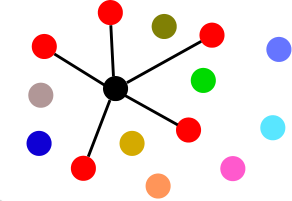
\includegraphics[width=0.6\textwidth]{images/sybil.png}
    \caption{I nodi rossi, controllati dall'attaccante, monopolizzano le comunicazioni del peer vittima (nero). \cite{owning}}
\end{figure}
Nel caso in cui i nodi implementino livelli di sicurezza più bassi di un \textit{full node} (i.e. \textit{SPV}) l'attaccante può anche generare delle transazioni invalide come transazioni \textit{coinbase} con un output maggiorato, utilizzo di \textit{UTXO} ed input errati.\newline
L'unico modo per riuscire nell'attacco è di controllare tutti i collegamenti nel tempo in cui nodo è online. Alcuni nodi non accettano richieste di connessione  e quindi è necessario che il nodo vittima richieda la connessione ai peer controllati dall'attaccante. Nel caso in cui invece sia possibile apportare un attacco di \textit{MITM} al nodo vittima la possibilità di successo è massima (le connessioni \textit{p2p} non sono cifrate o autenticate) ma la plausibilità di uno scenario simile è minima (l'attaccante deve aver compromesso la rete utilizzata dalla vittima o il sistema stesso).\newline
Una soluzione a questo tipo di attacco comporta la costruzione di una lista di nodi considerati sicuri ed onesti, aggiornata periodicamente, e evitare di utilizzare connessioni non sicure per transazioni online.\newline
Il software \texttt{bitcoind} accetta in totale $125$ connessioni di cui fino ad $8$ come canali di uscita e le restanti come ingressi. È stato inoltre progettato per evitare di connettersi in uscita a più di un \textit{IP} che nello stesso blocco (\texttt{/16}, fonte: \href{https://en.bitcoin.it/wiki/Weaknesses#Sybil_attack}{bitcoin.it}).

\section{Selfish Mining Attack}
Una volta che un miner è riuscito a trovare il \textit{nonce} corretto il blocco viene propagato nella rete ed accettato dagli altri peer come successivo nella catena.\newline
Una alternativa è quella di non pubblicare il blocco immediatamente ma iniziare a lavorare sul blocco successivo con l'obiettivo di calcolare due blocchi prima che il resto della rete ne abbia aggiunto uno. Se il miner riesce a creare una blockchain privata di due blocchi più lunga di quella pubblica, tutta l'energia e il tempo computazionale della restante rete risulta futile. Una volta che gli altri peer pubblicano il primo nodo l'attaccante può pubblicare contemporaneamente i due blocchi da lui calcolati. Una volta raggiunta la maggior parte dei peer i due blocchi pubblicati sono aggiunti alla blockchain che risulterà essere quella più lunga e valida. L'obiettivo è rendere inutile il resto della rete ed aumentare le possibilità di ottenere la ricompensa per il mining.
\begin{figure}[H]
    \centering
    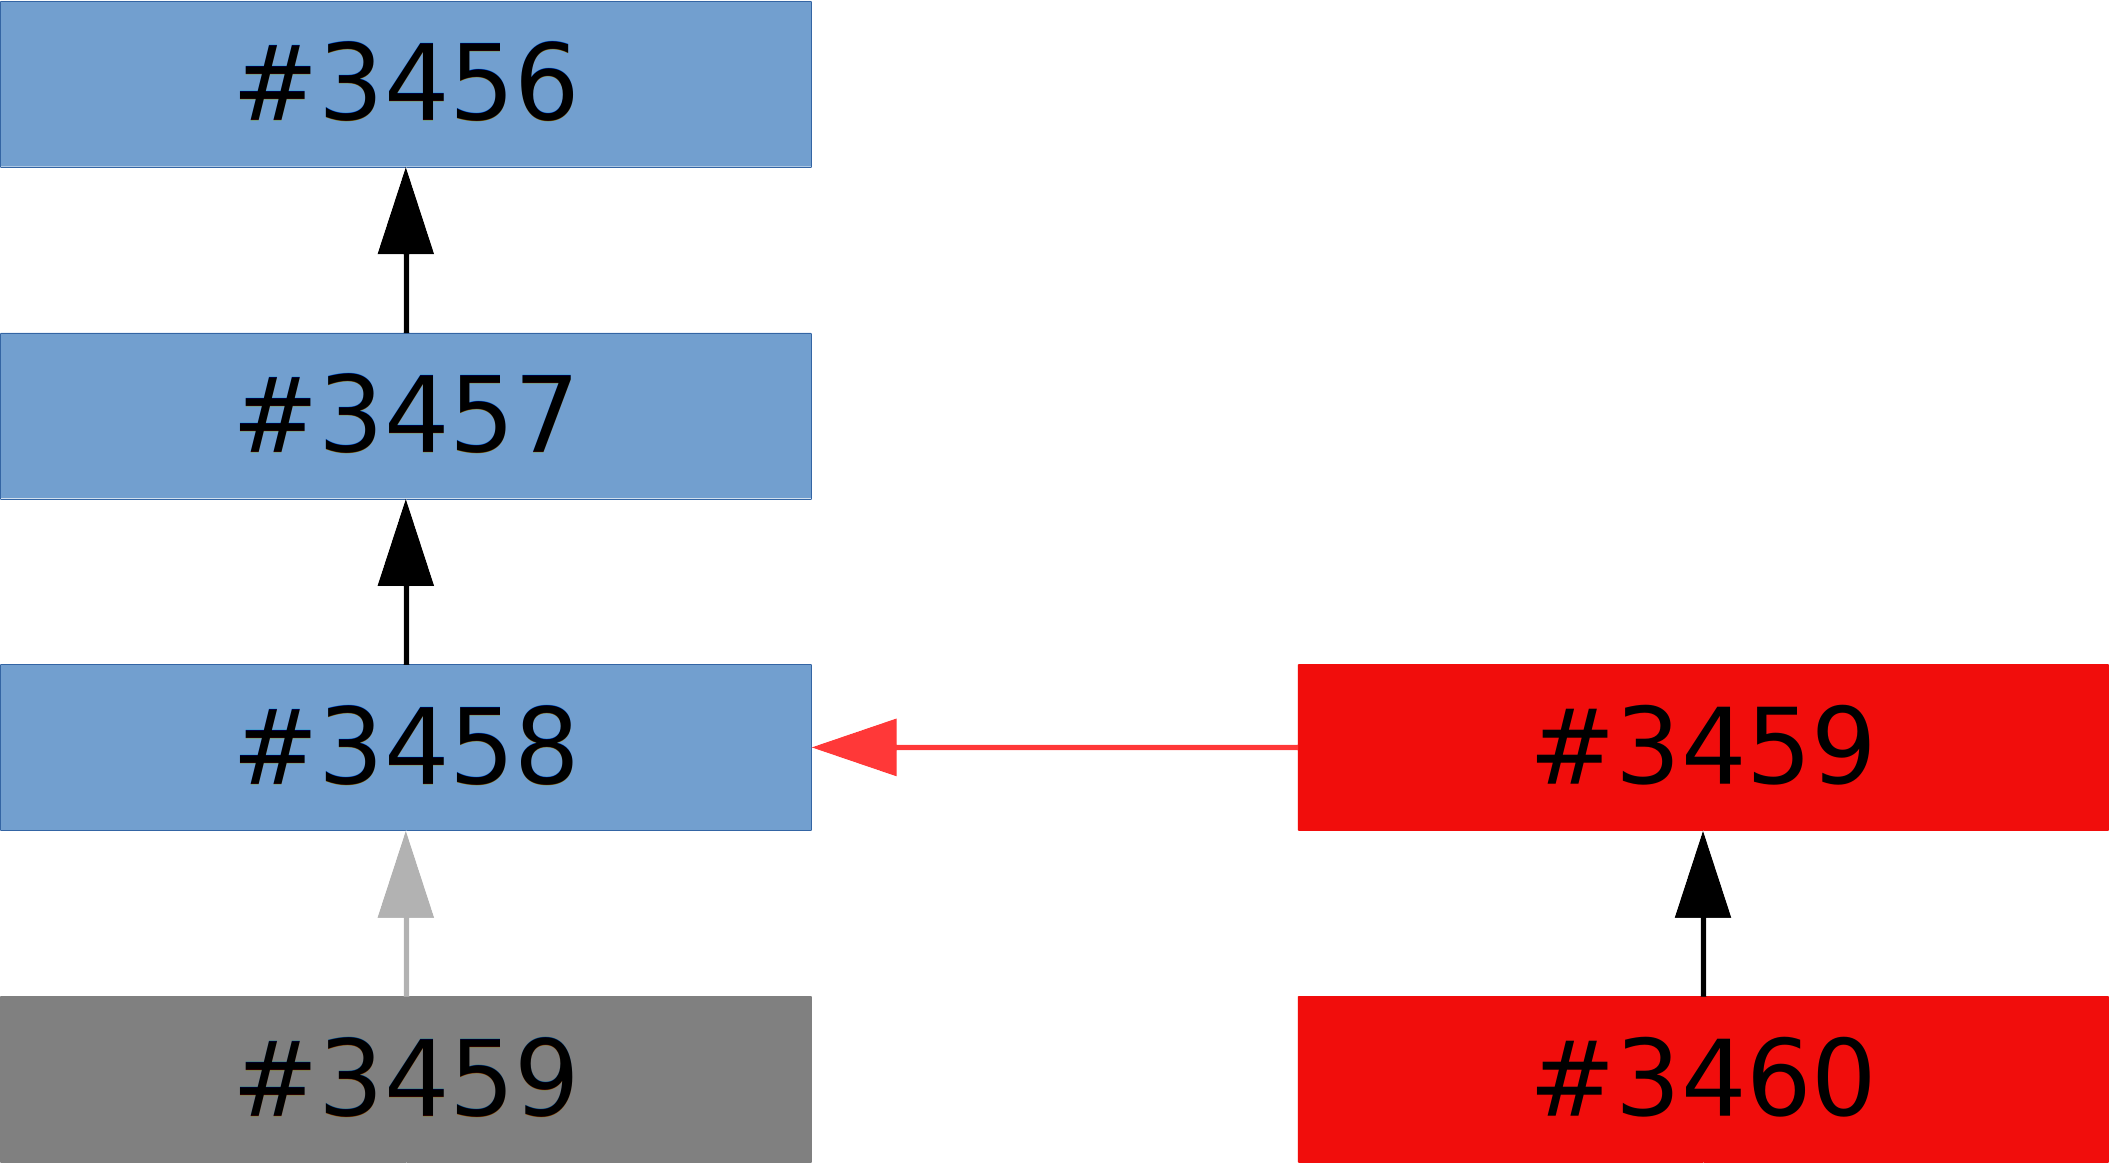
\includegraphics[width=0.6\textwidth]{images/selfish.png}
    \caption{Illustrazione di \textit{selfish mining}. L'attaccante riesce a calcolare i blocchi $3459$ e $3460$ (in rosso). Non appena la rete pubblica il blocco $3459$ (in grigio) l'attaccante diffonde i due blocchi precedentemente calcolati rendendo orfano il blocco $3459$ (in grigio).}
\end{figure}
La probabilità che però un singolo miner possa riuscire a trovare due blocchi consecutivi è molto bassa e quindi l'attaccante potrebbe decidere di pubblicare il primo blocco trovato non appena qualcun altro diffonde lo stesso blocco. Questo crea una \textit{fork} di un blocco che potrebbe avvantaggiare l'attaccante se gli altri miner decidessero di lavorare sulla sua \textit{branch}. Il successo dipende quindi non solo dalla potenza di calcolo ma anche dalla posizione nella rete.

\section{Attacchi alle transazioni}
Un possibile attacco apportato sul meccanismo delle transazioni è dovuto ad una vulnerabilità che alcune transazioni hanno: \textit{Transaction Malleability}.\newline
Le transazioni vengono identificate tramite un hash univoco ed unico; in questo modo è possibile creare una catena di transazioni e ricostruire la storia delle \textit{UTXO}. È possibile però cambiare questo identificativo una volta pubblicata la transazione se la signature inserita non è costruita utilizzando tutti i dati inseriti nella transazione. Una volta identificata una transazione \textit{malleabile} è possibile cambiarla in modo tale che l'hash sia invalido: output e input della transazione rimangono invariati. Il problema nasce dal fatto che non è possibile considerare sicura una catena di transazioni non ancora confermate e che possono essere soggette a modifiche. In aggiunta, ogni client deve sempre controllare che ci siano delle transazioni verso il proprio wallet e assumere che una \textit{UTXO} esista perché un altro utente l'ha creata non è considerato sicuro.\newline
La malleabilità è presente proprio nella signature e sono possibili diversi scenari in cui è possibile modificare dei dati:
\begin{itemize}
    \item l'encoding della signature può essere cambiato in quanto l'implementazione dell'encoder \texttt{DER} (\textit{Distinguished Encoding Rules}) è lasca e permette diverse rappresentazioni della signature codificata. Tramite \textit{BIP66} e quindi una \textit{soft fork} è stato imposto un controllo più stringente;
    \item è possibile inserire nuovi dati nello script di input: ad esempio una signature può essere inserita come somma di due numeri;
    \item utilizzare operatori per operazioni di \texttt{push} alternativi come \texttt{OP\_PUSHDATA1} o \texttt{OP\_PUSHDATA2};
    \item degli zero possono essere preposti ai valori inseriti producendo un valore equivalente;
    \item è possibile invertire i bit di parità inseriti nella signature (producendo un numero più grande) producendo una signature valida;
    \item è possibile anteporre dei dati inutili al fine dell'esecuzione all'inizio dello script. Lo stack a fine esecuzione presenta dei dati che non sono stati letti od utilizzati;
    \item dei dati possono essere aggiunti alla fine: uno script che inizia con l'operatore \texttt{OP\_DROP} scarta il valore in cima allo stack ovvero il risultato dello script. Il problema non è completamente risolvibile in quanto lo script di input deve inserire un elemento nullo;
    \item alcune signature supportano intenzionalmente delle modifiche successive;
\end{itemize}
Attualmente, però, quasi tutti gli scenari sono stati risolti tramite \href{https://en.bitcoin.it/wiki/BIP_0062}{\textit{BIP62}} e \href{https://en.bitcoin.it/wiki/BIP_0066}{\textit{BIP66}}.\newline
La malleabilità delle transazioni affligge solamente quelle transazioni che non sono ancora state inserite nella blockchain. Esistono alcuni scenari particolari per cui è possibile che si verifichi questa problematica.
\begin{figure}[H]
    \centering
    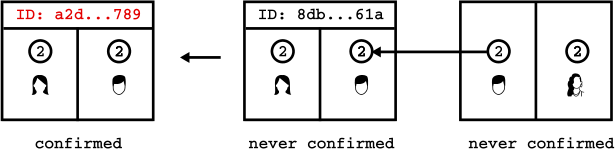
\includegraphics[width=\textwidth]{images/malleability.png}
    \caption{Alice versa a Bob alcuni \texttt{BTC} (centro) che Bob usa per pagare Carol (destra). La transazione di Alice viene però modificata e questa viene inserita nella blockchain (sinistra) rendendo orfane le altre due transazioni.\cite{owning}}
\end{figure}
Dato, per esempio, un pagamento di $2$ \texttt{BTC} da Alice a Bob, è possibile che Bob utilizzi quell'input per una nuova transazione verso Carol. Prima che entrambe le transazioni siano inserite nella blockchain, una transazione, modificata, viene inserita nella blockchain prima delle altre. In questo modo nessuna delle due transazioni può essere inserita nella blockchain in quanto non hanno degli identificativi validi.\newline
Un altro scenario di utilizzo della malleabilità in maniera malevola è ingannare un utente facendogli credere che una transazione non sia stata ricevuta. Bob decide di ritirare i Bitcoin che ha depositato in un exchange controllato da Alice. L'exchange deve, quindi, inviare una transazione al wallet di Bob che però convince Alice di non aver mai ricevuto il denaro e produce una copia modificata della transazione producendo un hash diverso. Alice, quindi, convinta che la transazione non abbia avuto successo, ne crea una nuova. Se la transazione, modificata da Bob, viene inserita nella blockchain prima delle altre verrà considerata valida e Bob potrà reclamare di non aver ancora ricevuto i Bitcoin. A questo punto Alice è costretta ad immettere una nuova transazione nella rete e perdere quindi altre monete.\newline
Ad inizio 2014, subito prima delle due \textit{BIP}, è stato rilevato un utilizzo massivo di questa vulnerabilità per eseguire un attacco \textit{DDoS} all'exchange di criptomonete \textit{Bitstamp}. Tramite dei \textit{bot}\footnote{Un bot, nel suo caso generico, è un software automatizzato per eseguire dei task semplici e ripetitivi. Nella connotazione malevola i bot sono il risultato una precedente compromissione tramite virus o worm. L'obiettivo è infettare il più dispositivi possibili per aumentare il raggio di azione e computazione di bot.} malevoli tutte le transazioni create, parallelamente venivano modificate e pubblicate sulla rete creando duplicati malformati producendo un notevole traffico e consumo di risorse nell'intera rete.

% NeoTex: mainfile=main.tex:
